\providecommand{\main}{../../..}
\documentclass[\main/main.tex]{subfiles}
\begin{document}

\subsection{Exercise 2}
Define briefly what is a \textbf{problem of mathematical programming}.

Given the following problem of mathematical programming:

\begin{align*}
  \min f(x) = 2x_1 + x_2                   \\
  g_1(x) = x_1^2 - 2x_1 - x_2 + 1 & \leq 0 \\
  g_2(x) = x_1^2 - 2x_1 + x_2 -1  & \leq 0 \\
  g_3(x) = -x_1                   & \leq 0
\end{align*}
\begin{enumerate}[a)]
  \item Represent the problem graphically.
  \item Determine candidates points according to the KKT conditions, in particular those of global minimum.
\end{enumerate}

\subsection{Exercise 2 resolution}
\subsubsection*{Problem of mathematical programming}
A problem of mathematical programming is the simplest kind of decision problem:

\begin{enumerate}
  \item The preference relationship $\Pi$ holds a known value function.
  \item The system is deterministic, meaning there's only one scenery.
  \item There's only one decision maker.
\end{enumerate}

\subsubsection*{Graphical representation}
\begin{figure}
  \begin{subfigure}{0.49\textwidth}
    \xygraph{0}{2}{0}{2}{0}{
      x^2 - 2*x - y +1 <=0 &&
      x^2 - 2*x + y -1 <=0
    }{2*x+y}
  \end{subfigure}
  \begin{subfigure}{0.49\textwidth}
    \includegraphics[width=0.9\textwidth]{20180124_02}
  \end{subfigure}
\end{figure}

\subsubsection*{Irregular points}

\paragraph*{Gradients}

\[
  \nabla f_1 = \begin{bmatrix}
    2 \\
    1
  \end{bmatrix}
  \qquad
  \nabla g_1 = \begin{bmatrix}
    2x_1 -2 \\
    -1
  \end{bmatrix}
  \qquad
  \nabla g_2 = \begin{bmatrix}
    2x_1 -2 \\
    1
  \end{bmatrix}
  \qquad
  \nabla g_3 = \begin{bmatrix}
    -1 \\
    0
  \end{bmatrix}
\]
The gradients are never equal to zero.

\paragraph*{Constraints intersections}

\[
  \begin{cases}
    g_1(x) = x_1^2 - 2x_1 - x_2 + 1 = 0 \\
    g_2(x) = x_1^2 - 2x_1 + x_2 -1  = 0
  \end{cases}
  \Rightarrow
  \begin{cases}
    x_1 = 0 \\
    x_2 = 1
  \end{cases}
  \lor
  \quad
  \begin{cases}
    x_1 = 2 \\
    x_2 = 1
  \end{cases}
\]

\[
  \begin{cases}
    g_1(x) = x_1^2 - 2x_1 - x_2 + 1 = 0 \\
    g_2(x) = x_1^2 - 2x_1 + x_2 -1  = 0 \\
    g_3(x) = -x_1                   = 0
  \end{cases}
  \Rightarrow
  \begin{cases}
    x_1 = 0 \\
    x_2 = 1
  \end{cases}
\]
The point $A = \rnd(0,1)$ is irregular for 2 reasons:
\begin{enumerate}
  \item The gradients matrix is singular in $A$.
  \item There are more constraints active in $A$ than there are variables.
\end{enumerate}

Therefore, $A$ is a candidate point.

\subsubsection*{KKT conditions}

\paragraph*{Lagrangian relaxation}

\[
  L(\bmx) = \begin{bmatrix}
    2 \\
    1
  \end{bmatrix} + \mu_1 \begin{bmatrix}
    2x_1 -2 \\
    -1
  \end{bmatrix} + \mu_2 \begin{bmatrix}
    2x_1 -2 \\
    1
  \end{bmatrix} + \mu_3 \begin{bmatrix}
    -1 \\
    0
  \end{bmatrix}
\]

\paragraph*{System of the KKT conditions}

\[
  \begin{cases}
    L(\bmx) = \begin{bmatrix}
      2 \\
      1
    \end{bmatrix} + \mu_1 \begin{bmatrix}
      2x_1 -2 \\
      -1
    \end{bmatrix} + \mu_2 \begin{bmatrix}
      2x_1 -2 \\
      1
    \end{bmatrix} + \mu_3 \begin{bmatrix}
      -1 \\
      0
    \end{bmatrix} = 0 \\
    \mu_1(x_1^2 - 2x_1 - x_2 + 1) = 0                                                                                                                 \\
    \mu_2(x_1^2 - 2x_1 + x_2 -1 ) = 0                                                                                                                 \\
    \mu_3(-x_1                  ) = 0                                                                                                                 \\
    x_1^2 - 2x_1 - x_2 + 1          \leq 0                                                                                                            \\
    x_1^2 - 2x_1 + x_2 -1           \leq 0                                                                                                            \\
    -x_1                            \leq 0                                                                                                            \\
    \mu_1 \geq 0                                                                                                                                      \\
    \mu_2 \geq 0                                                                                                                                      \\
    \mu_3 \geq 0
  \end{cases}
\]
\paragraph*{Search tree}
We begin the search tree with $\mu_1$:

\begin{figure}
  \begin{tikzpicture}
    \Tree[.\text{root}
      [.$\mu_1=0$ ]
      [.$\mu_1>0$ ]
    ]
  \end{tikzpicture}
  \caption{Search tree, step 1}
\end{figure}

\paragraph*{Case $\mu_1=0$}
\[
  \begin{cases}
    L(\bmx) = \begin{bmatrix}
      2 \\
      1
    \end{bmatrix} + \mu_2 \begin{bmatrix}
      2x_1 -2 \\
      1
    \end{bmatrix} + \mu_3 \begin{bmatrix}
      -1 \\
      0
    \end{bmatrix} = 0 \\
    \mu_2(x_1^2 - 2x_1 + x_2 -1 ) = 0                                                                              \\
    \mu_3(-x_1                  ) = 0                                                                              \\
    x_1^2 - 2x_1 - x_2 + 1          \leq 0                                                                         \\
    x_1^2 - 2x_1 + x_2 -1           \leq 0                                                                         \\
    -x_1                            \leq 0                                                                         \\
    \mu_1 = 0                                                                                                      \\
    \mu_2 \geq 0                                                                                                   \\
    \mu_3 \geq 0
  \end{cases}
  \Rightarrow
  \error{\mu_2 = -1}
\]
If we add the constrain $\mu_1=0$ the system becomes impossible.

\paragraph*{Case $\mu_1>0$}

\begin{figure}
  \begin{tikzpicture}
    \Tree[.\text{root}
      [.$\mu_1=0$
        [.$\error{\mu_2 = -1}$ ]
      ]
      [.$\mu_1>0$
        [.$\mu_2=0$ ]
          [.$\mu_2>0$ ]
      ]
    ]
  \end{tikzpicture}
  \caption{Search tree, step 2}
\end{figure}

\subparagraph*{Case $\mu_2=0$}

\[
  \begin{cases}
    L(\bmx) = \begin{bmatrix}
      2 \\
      1
    \end{bmatrix} + \mu_1 \begin{bmatrix}
      2x_1 -2 \\
      -1
    \end{bmatrix} + \mu_3 \begin{bmatrix}
      -1 \\
      0
    \end{bmatrix} = 0 \\
    \mu_1(x_1^2 - 2x_1 - x_2 + 1) = 0                                                                              \\
    \mu_3(-x_1                  ) = 0                                                                              \\
    x_1^2 - 2x_1 - x_2 + 1          \leq 0                                                                         \\
    x_1^2 - 2x_1 + x_2 -1           \leq 0                                                                         \\
    -x_1                            \leq 0                                                                         \\
    \mu_1 > 0                                                                                                      \\
    \mu_2 = 0                                                                                                      \\
    \mu_3 \geq 0
  \end{cases}
  \Rightarrow
  \begin{cases}
    x_2 = 1   \\
    x_1 = 0   \\
    \mu_1 = 1 \\
    \mu_2 = 0 \\
    \mu_3 = 0
  \end{cases}
\]
We identify again the same candidate point, $A = (0,1)$.

\subparagraph*{Case $\mu_2>0$}
\[
  \begin{cases}
    L(\bmx) = \begin{bmatrix}
      2 \\
      1
    \end{bmatrix} + \mu_1 \begin{bmatrix}
      -2 \\
      -1
    \end{bmatrix} + \mu_2 \begin{bmatrix}
      -2 \\
      1
    \end{bmatrix} + \mu_3 \begin{bmatrix}
      -1 \\
      0
    \end{bmatrix} = 0 \\
    x_1                           = 0                                                                                                                 \\
    x_2                           = 1                                                                                                                 \\
    \mu_1 > 0                                                                                                                                         \\
    \mu_2 > 0                                                                                                                                         \\
    \mu_3 \geq 0
  \end{cases}
  \lor
  \quad
  \begin{cases}
    L(\bmx) = \begin{bmatrix}
      2 \\
      1
    \end{bmatrix} + \mu_1 \begin{bmatrix}
      2 \\
      -1
    \end{bmatrix} + \mu_2 \begin{bmatrix}
      2 \\
      1
    \end{bmatrix} = 0 \\
    x_1                           = 2                                                                              \\
    x_2                           = 1                                                                              \\
    \mu_1 > 0                                                                                                      \\
    \mu_2 > 0                                                                                                      \\
    \mu_3 = 0
  \end{cases}
  \Rightarrow
  \error{\mu_2 = -1}
\]
We expand over $\mu_3$.

\begin{figure}
  \begin{tikzpicture}
    \Tree[.\text{root}
      [.$\mu_1=0$
        [.$\error{\mu_2 = -1}$ ]
      ]
      [.$\mu_1>0$
        [.$\mu_2=0$
            [.$A=(0,1)$ ]
          ]
          [.$\mu_2>0$
            [.$x_1=0,x_2=1$
                [.$\mu_3=0$ ]
                  [.$\mu>0$ ]
              ]
              [.$x_1=2,x_2=1,\mu_3=0$
                [.$\error{\mu_2=-1}$ ]
              ]
          ]
      ]
    ]
  \end{tikzpicture}
  \caption{Search tree, step 3}
\end{figure}

\subparagraph*{Case $\mu_3=0$}
\[
  \begin{cases}
    L(\bmx) = \begin{bmatrix}
      2 \\
      1
    \end{bmatrix} + \mu_1 \begin{bmatrix}
      -2 \\
      -1
    \end{bmatrix} + \mu_2 \begin{bmatrix}
      -2 \\
      1
    \end{bmatrix}  = 0 \\
    x_1                           = 0                                                                               \\
    x_2                           = 1                                                                               \\
    \mu_1 > 0                                                                                                       \\
    \mu_2 > 0                                                                                                       \\
    \mu_3 = 0
  \end{cases}
  \Rightarrow
  \error{\mu_2=0 \land \mu_2>0}
\]
\begin{figure}
  \begin{tikzpicture}
    \Tree[.\text{root}
      [.$\mu_1=0$
        [.$\error{\mu_2 = -1}$ ]
      ]
      [.$\mu_1>0$
        [.$\mu_2=0$
            [.$A=(0,1)$ ]
          ]
          [.$\mu_2>0$
            [.$x_1=0,x_2=1$
                [.$\mu_3=0$
                    [.$\error{\mu_2=0 \land \mu_2>0}$ ]
                  ]
                  [.$\mu>0$ ]
              ]
              [.$x_1=2,x_2=1,\mu_3=0$
                [.$\error{\mu_2=-1}$ ]
              ]
          ]
      ]
    ]
  \end{tikzpicture}
  \caption{Search tree, step 3}
\end{figure}

\subparagraph*{Case $\mu_3>0$}
\[
  \begin{cases}
    L(\bmx) = \begin{bmatrix}
      2 \\
      1
    \end{bmatrix} + \mu_1 \begin{bmatrix}
      -2 \\
      -1
    \end{bmatrix} + \mu_2 \begin{bmatrix}
      -2 \\
      1
    \end{bmatrix} + \mu_3 \begin{bmatrix}
      -1 \\
      0
    \end{bmatrix} = 0 \\
    x_1                           = 0                                                                                                                 \\
    x_2                           = 1                                                                                                                 \\
    \mu_1 > 0                                                                                                                                         \\
    \mu_2 > 0                                                                                                                                         \\
    \mu_3 > 0
  \end{cases}
  \Rightarrow
  \error{-4\mu_1 - \mu_3 = 0 \land \mu_1 > 0 \land \mu_3 > 0}
\]
\begin{figure}
  \begin{tikzpicture}
    \Tree[.\text{root}
      [.$\mu_1=0$
        [.$\error{\mu_2 = -1}$ ]
      ]
      [.$\mu_1>0$
        [.$\mu_2=0$
            [.$A=(0,1)$ ]
          ]
          [.$\mu_2>0$
            [.$x_1=0,x_2=1$
                [.$\mu_3=0$
                    [.$\error{\mu_2=0 \land \mu_2>0}$ ]
                  ]
                  [.$\mu>0$
                    [.$\error{-4\mu_1 - \mu_3 = 0 \land \mu_1 > 0 \land \mu_3 > 0}$ ]
                  ]
              ]
              [.$x_1=2,x_2=1,\mu_3=0$
                [.$\error{\mu_2=-1}$ ]
              ]
          ]
      ]
    ]
  \end{tikzpicture}
  \caption{Search tree, ended}
\end{figure}

The only candidate point is $A=(0,1)$, with value $z=1$.
\end{document}